\subsection{Building blocks}
\begin{frame}
\frametitle{Findings}
\framesubtitle{Building blocks}
\begin{table}
\begin{tabular}{p{7cm}p{3cm}}
\begin{itemize}
  \item DHT based (Pastry)
  \item Each node has its own pair of Pub/Priv keys
  \item Simple storage system
  \item Reputation system (WTR + CORPS)
  \item Challenges and computational puzzles
    % CORPS builds a double ring inside the DHT to find the most trustworthy node to a key K
  \item System protocols
\end{itemize}
&
\vspace{1.5cm}

\includegraphics[width=4cm]{img/example}\\
\end{tabular}
\end{table}
\end{frame}

\subsection{System protocols}
\begin{frame}
\frametitle{System protocols}
%\framesubtitle{Building blocks}
\begin{table}
\begin{tabular}{p{7cm}p{3cm}}
\begin{itemize}
  \item Securing the nodes of a leafset
  \item Account registration
  \item User sign in
  \item Logout
  \item Password Change
  \item User private key recovery
\end{itemize}
&
\vspace{1.5cm}

\includegraphics[width=4cm]{img/example}\\
\end{tabular}
\end{table}
\end{frame}

\subsection{Securing the nodes of a leafset}
\begin{frame}
\frametitle{System protocols}
\framesubtitle{Securing the nodes of a leafset}
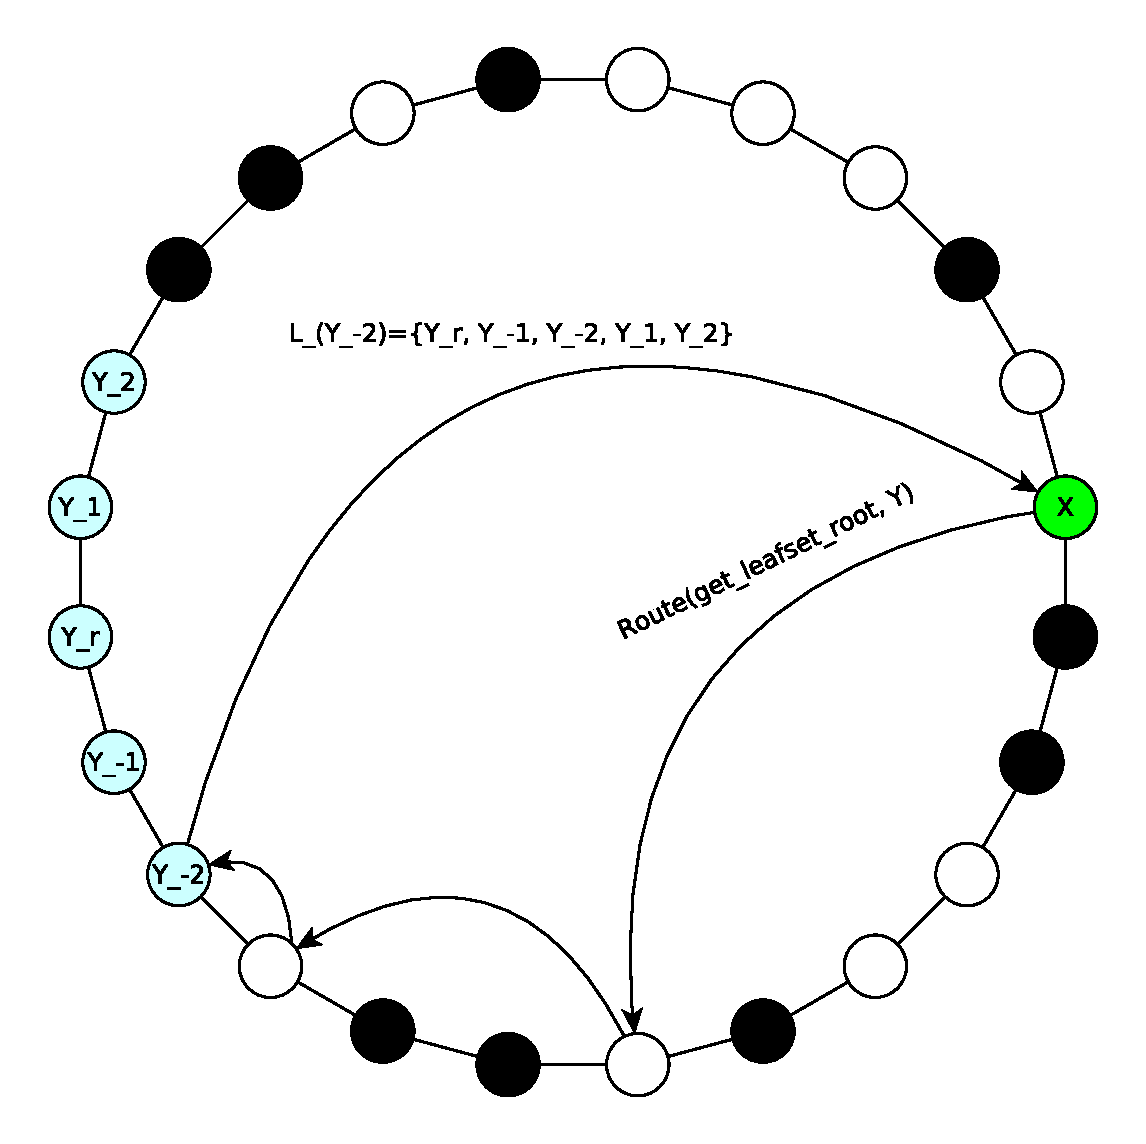
\includegraphics[height=0.7\textheight]{../../img/secure_routing}\\
%\begin{table}
%\begin{tabular}{p{7cm}p{3cm}}
%&
%\vspace{1.5cm}
%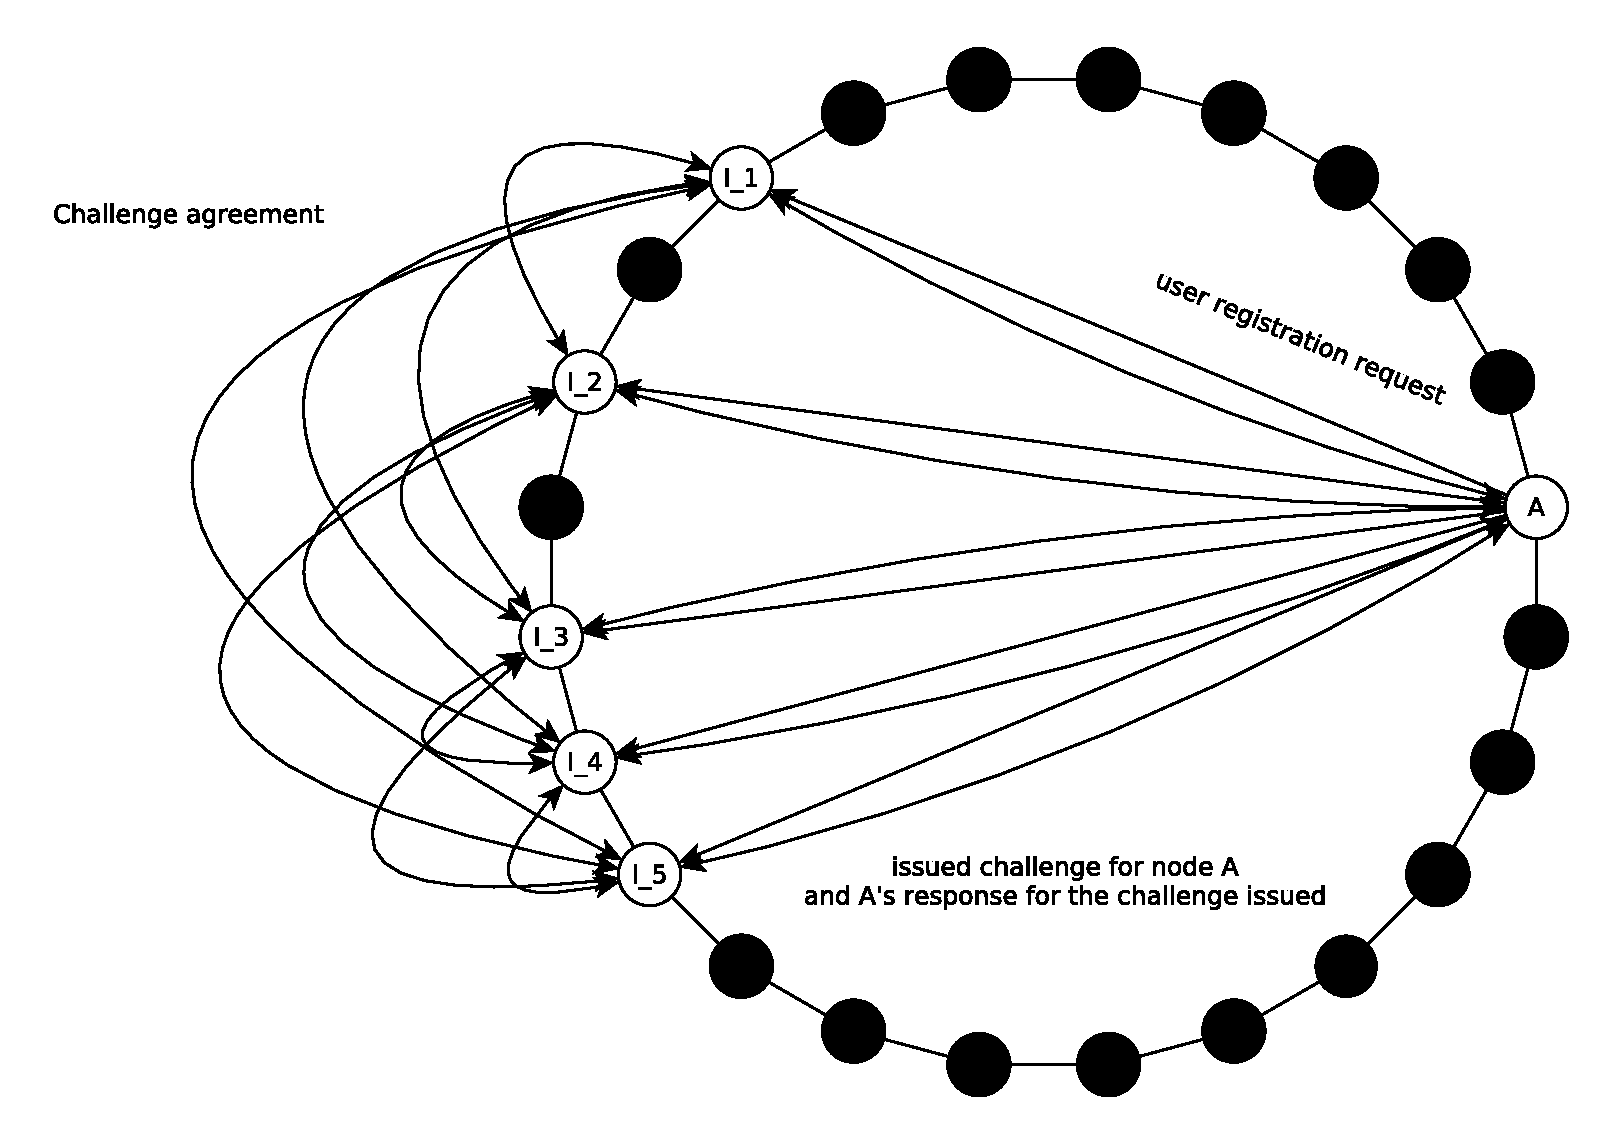
\includegraphics[width=4cm]{../../img/sign_up}\\
%\end{tabular}
%\end{table}
\end{frame}

\subsection{Account registration}
\begin{frame}
\frametitle{System protocols}
\framesubtitle{Account Registration}
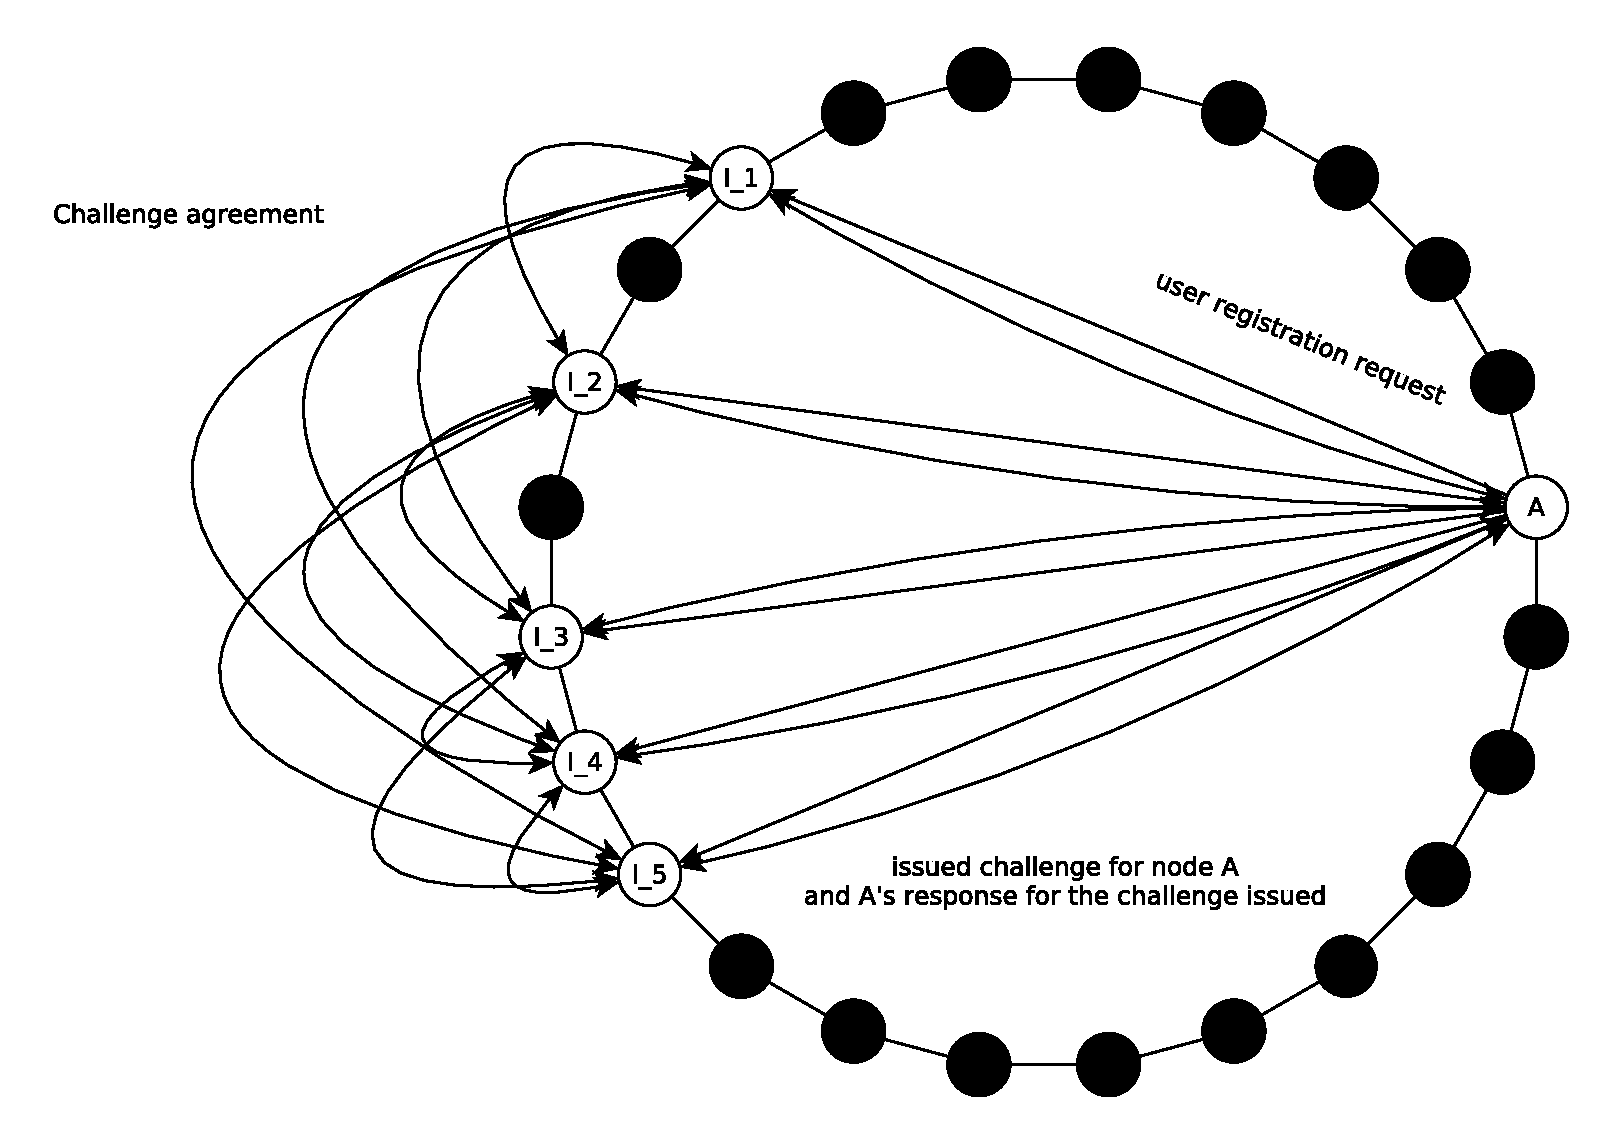
\includegraphics[height=0.7\textheight]{../../img/sign_up}\\
%\begin{table}
%\begin{tabular}{p{7cm}p{3cm}}
%&
%\vspace{1.5cm}
%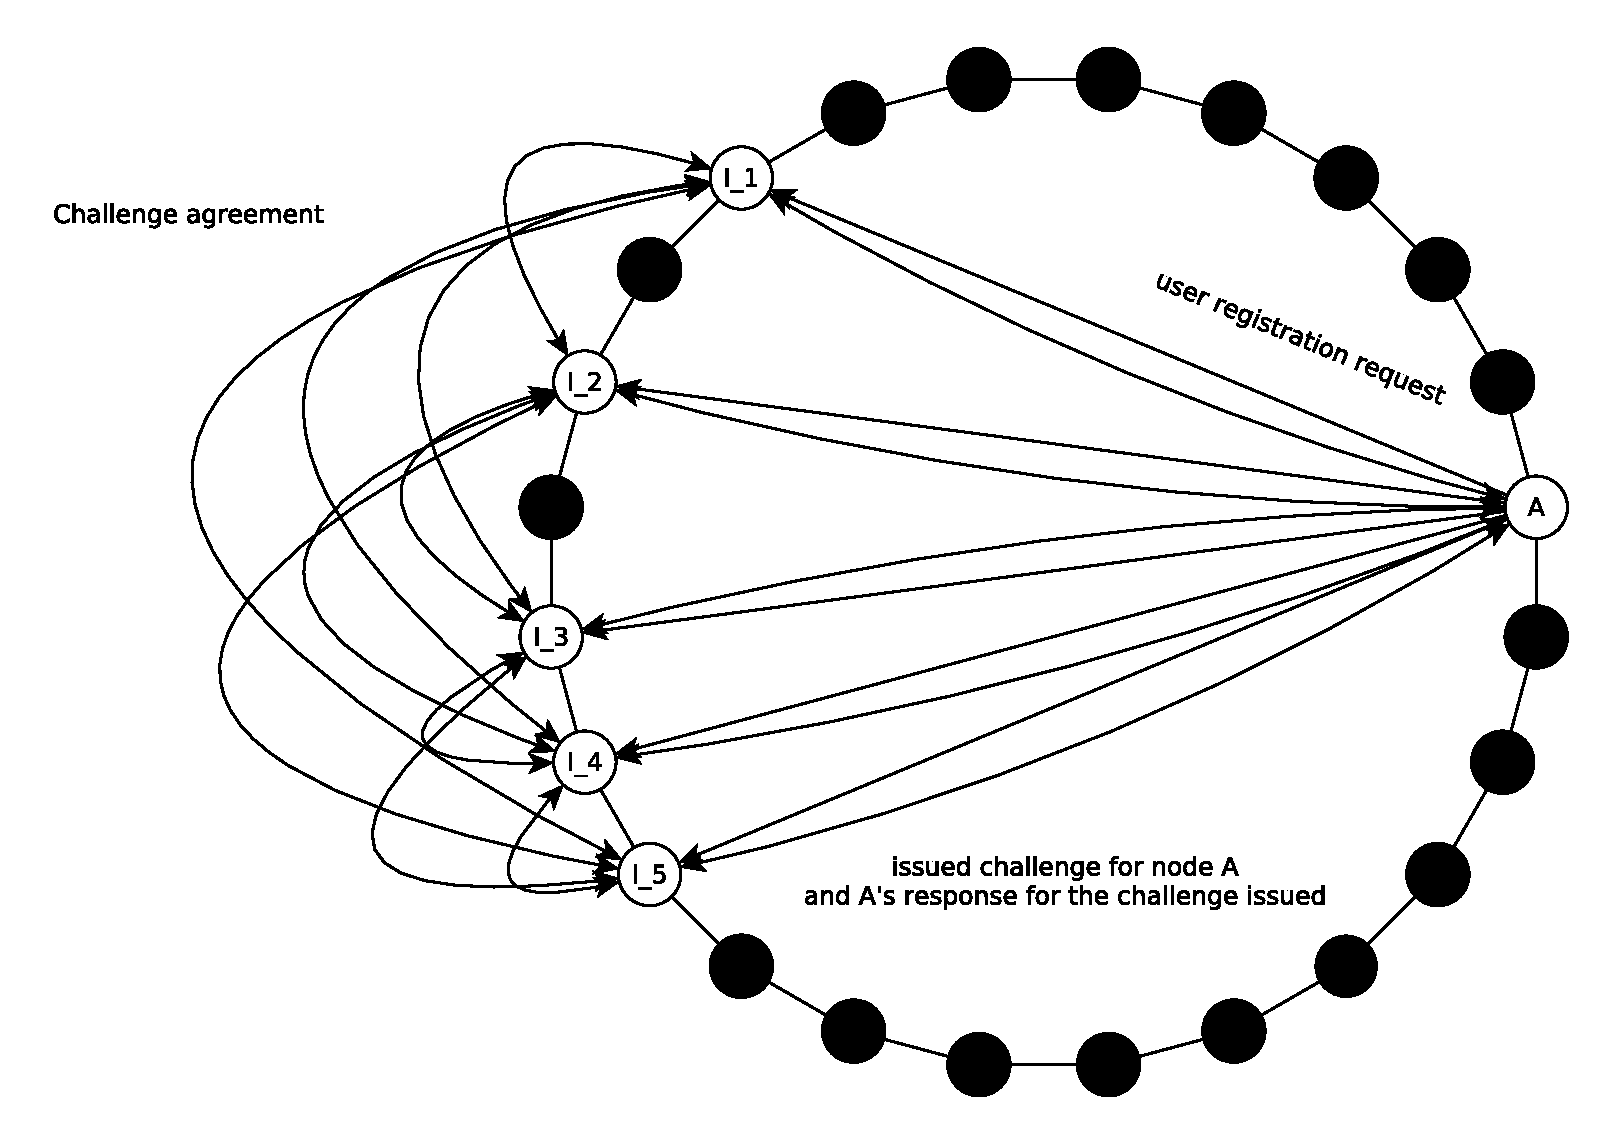
\includegraphics[width=4cm]{../../img/sign_up}\\
%\end{tabular}
%\end{table}
\end{frame}

\subsection{User sign in}
\begin{frame}
\frametitle{System protocols}
\framesubtitle{User sign in (Start)}
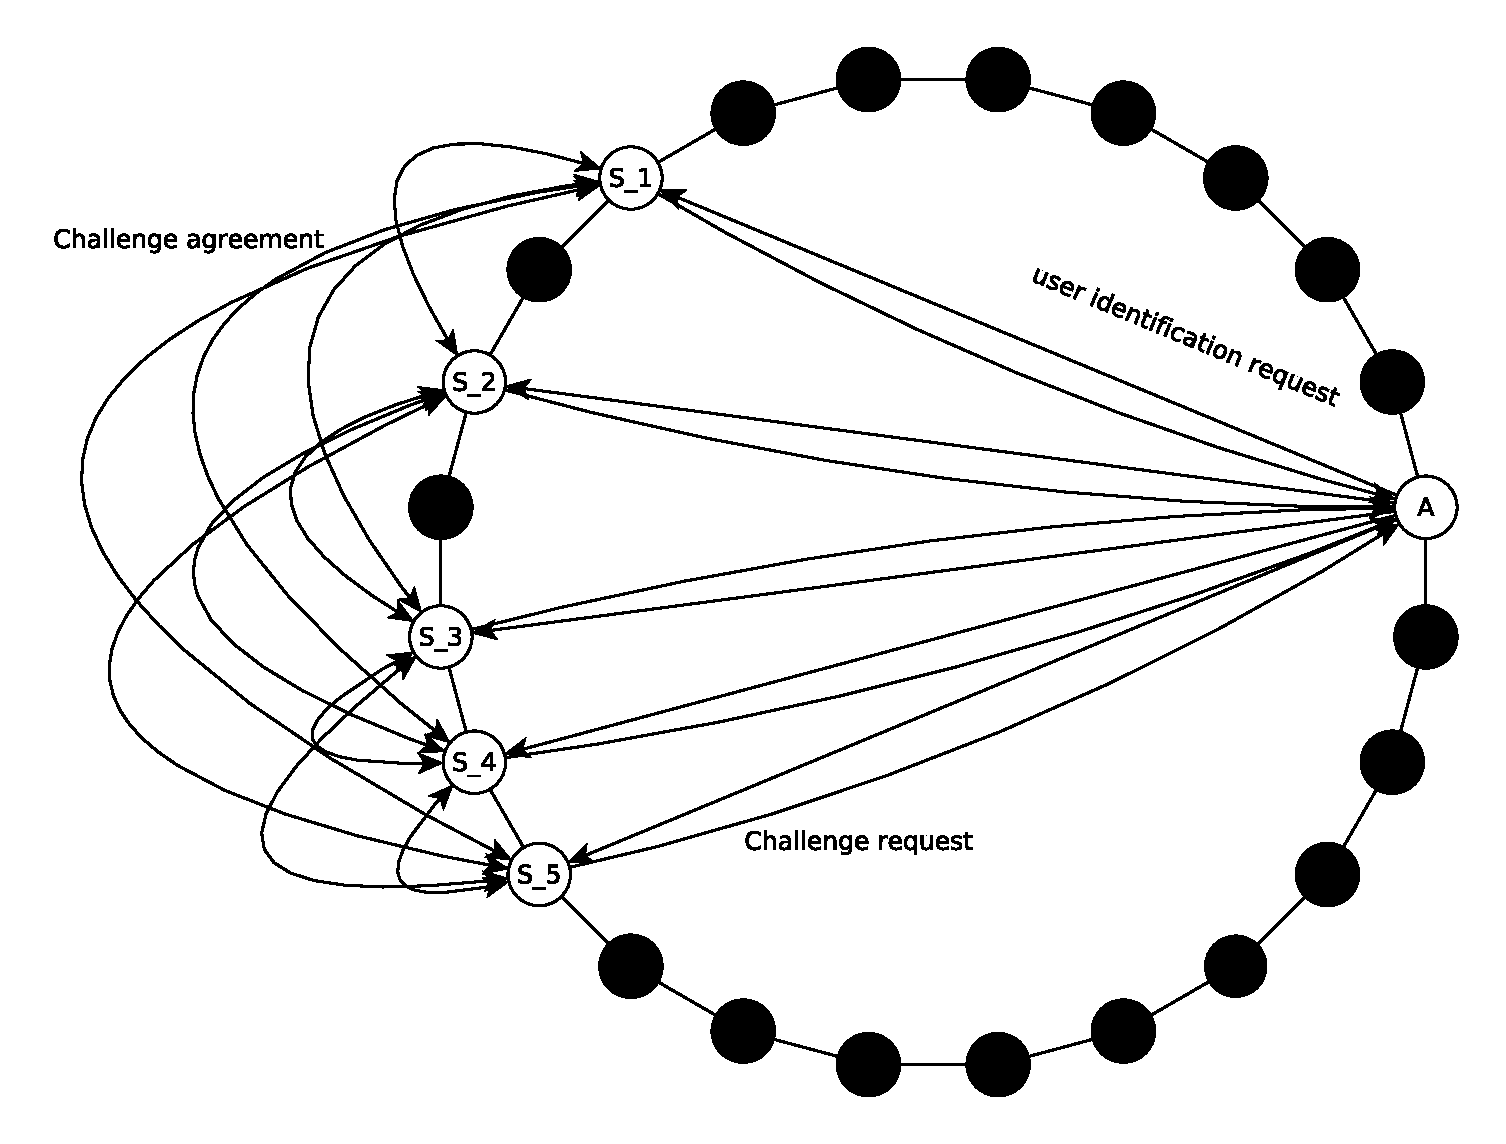
\includegraphics[height=0.7\textheight]{../../img/sign_in}\\
%\begin{table}
%\begin{tabular}{p{7cm}p{3cm}}
%&
%\vspace{1.5cm}
%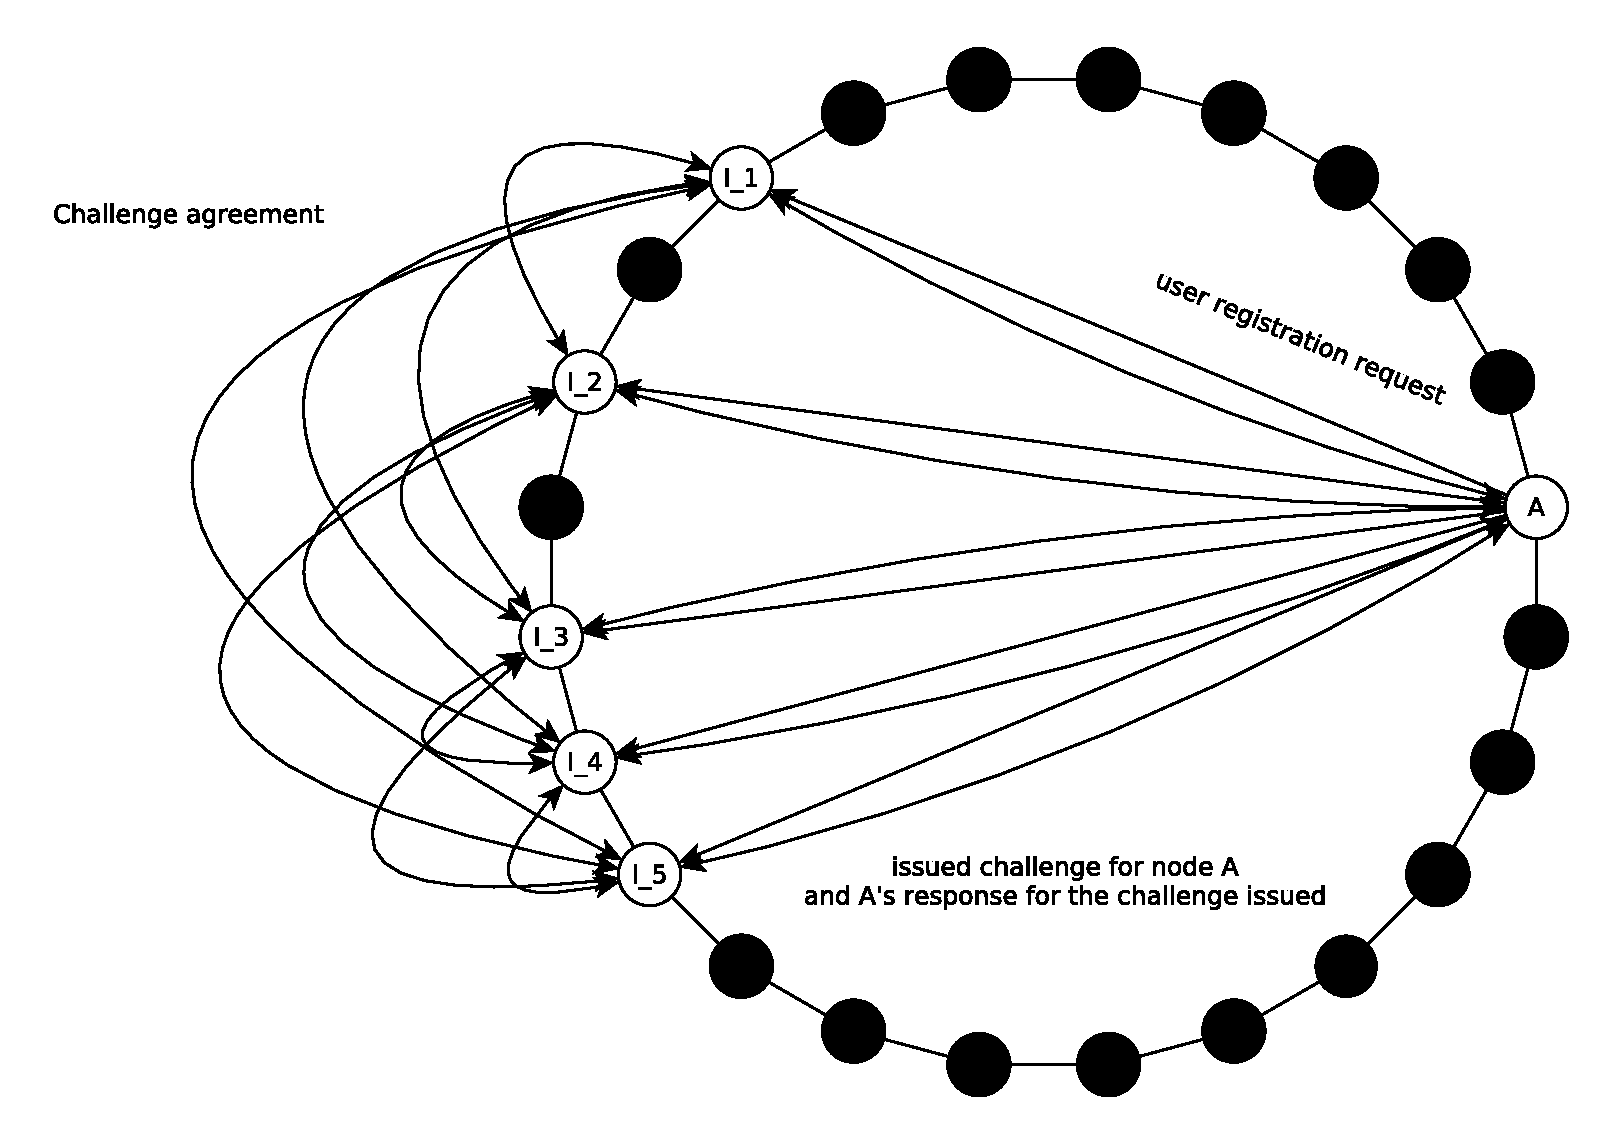
\includegraphics[width=4cm]{../../img/sign_up}\\
%\end{tabular}
%\end{table}
\end{frame}

\begin{frame}
\frametitle{System protocols}
\framesubtitle{User sign in (Retrieve of public key)}
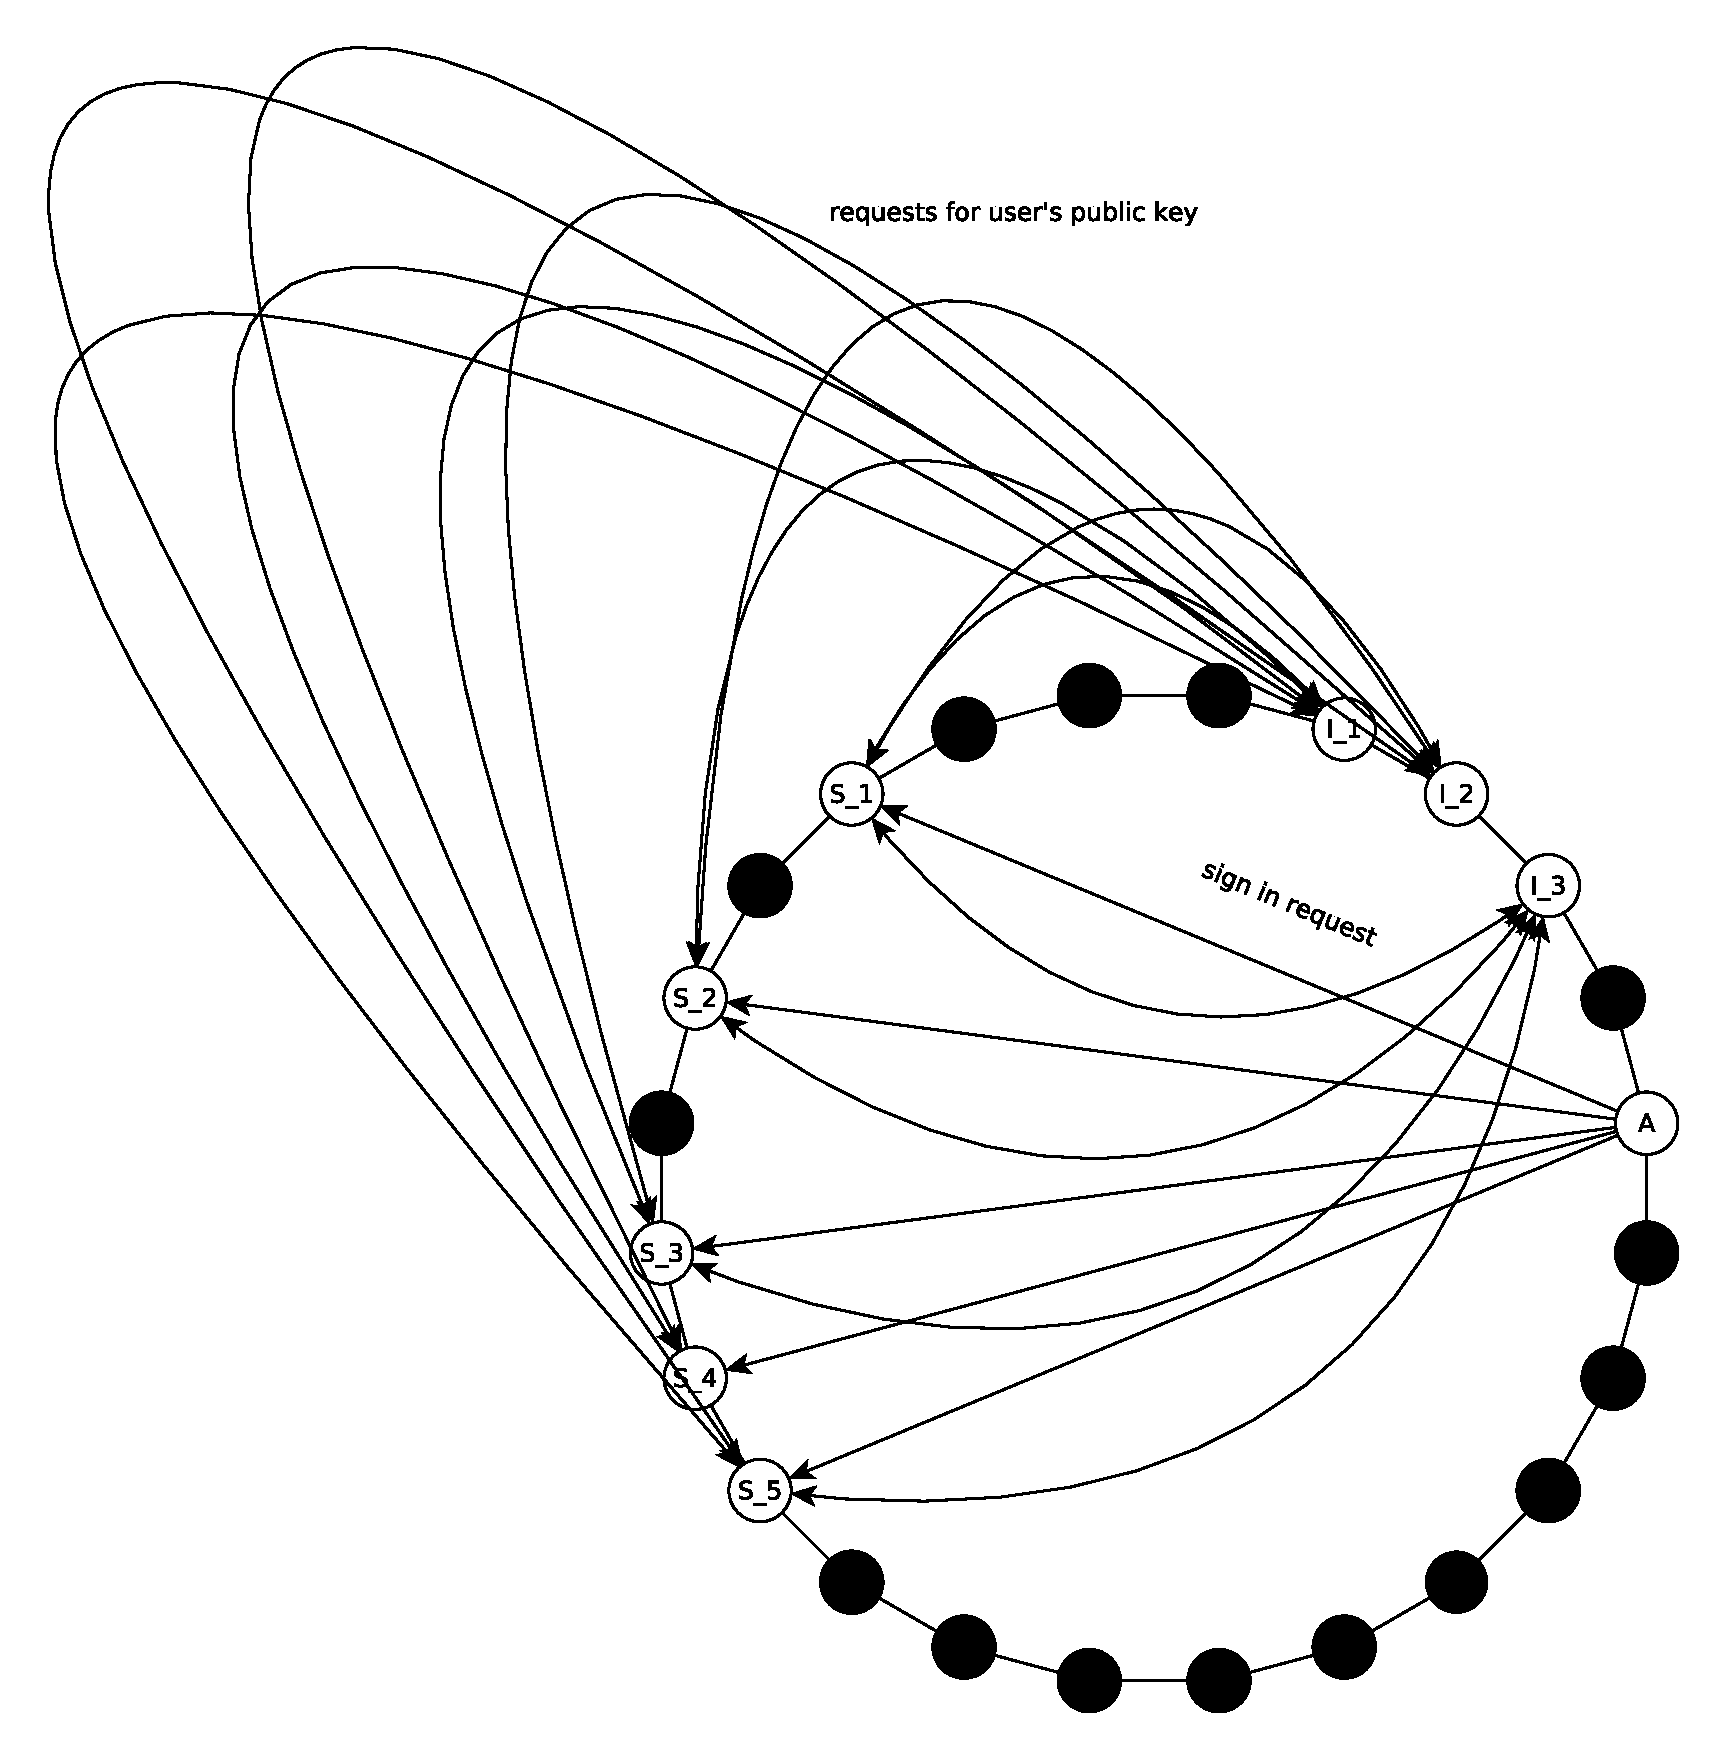
\includegraphics[height=0.7\textheight]{../../img/sign_in_2}
%\begin{table}
%\begin{tabular}{p{7cm}p{3cm}}
%&
%\vspace{1.5cm}
%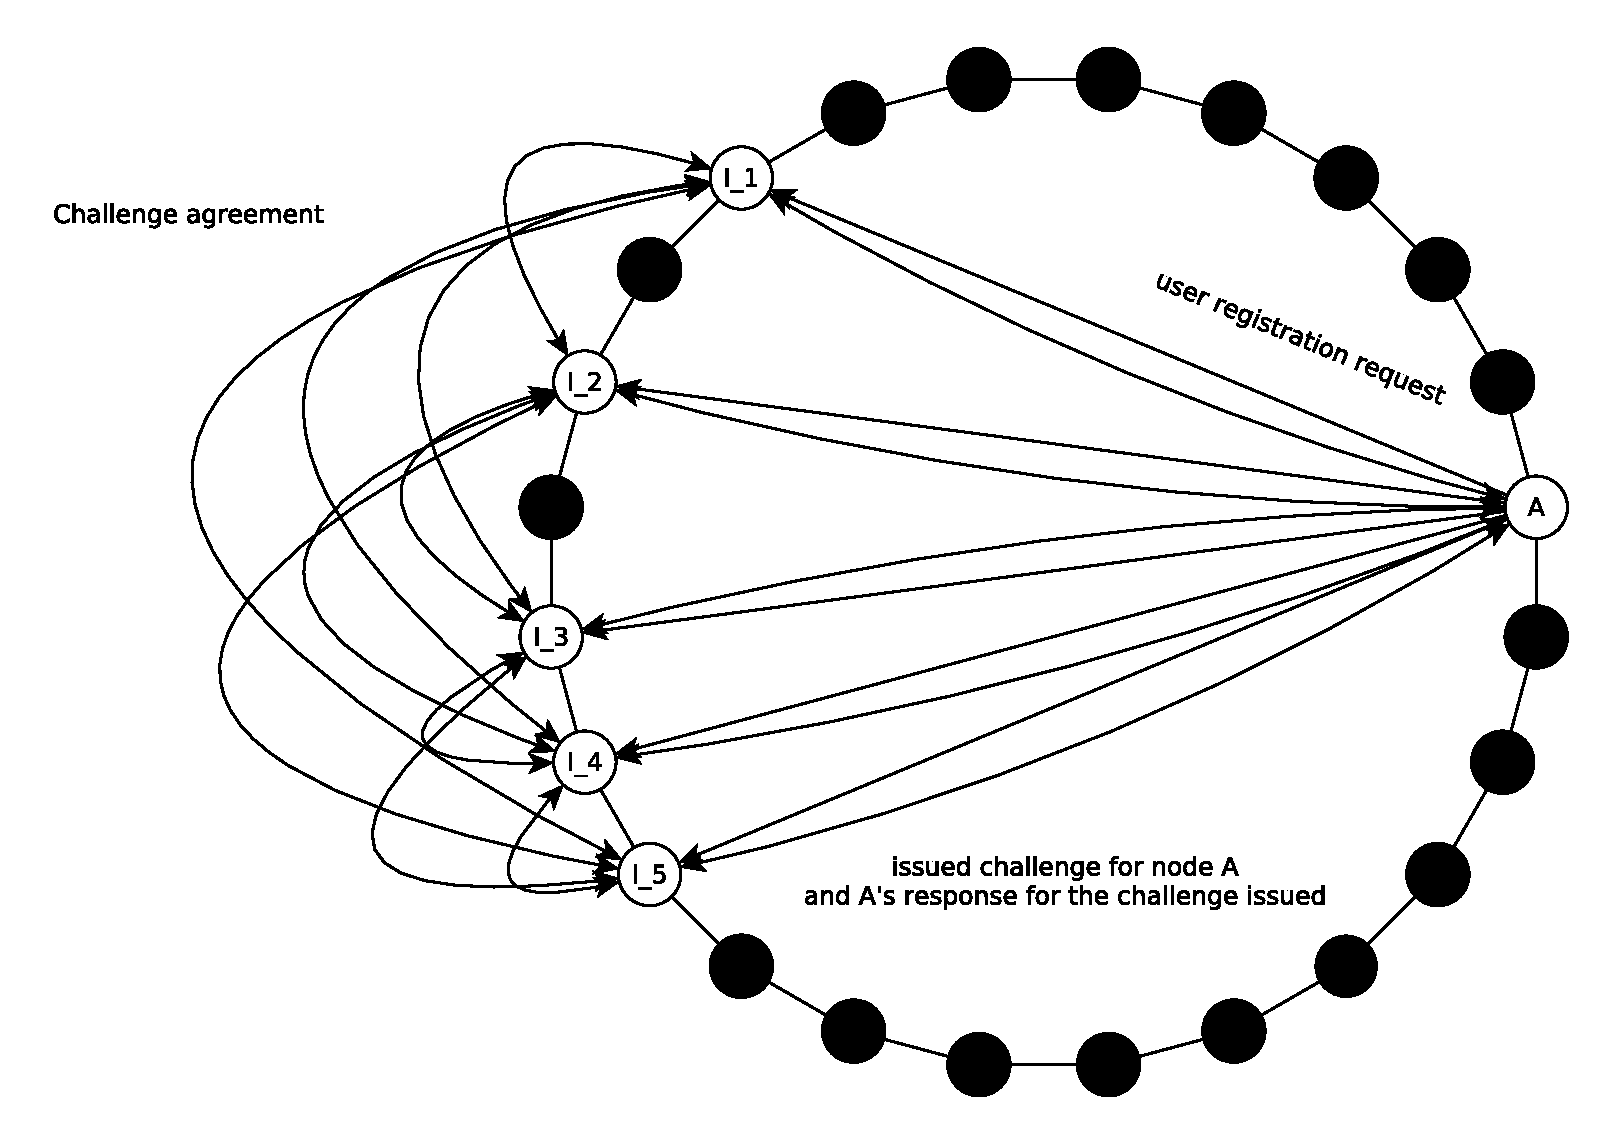
\includegraphics[width=4cm]{../../img/sign_up}\\
%\end{tabular}
%\end{table}
\end{frame}

\begin{frame}
\frametitle{System protocols}
\framesubtitle{User sign in (Generation of session keys)}
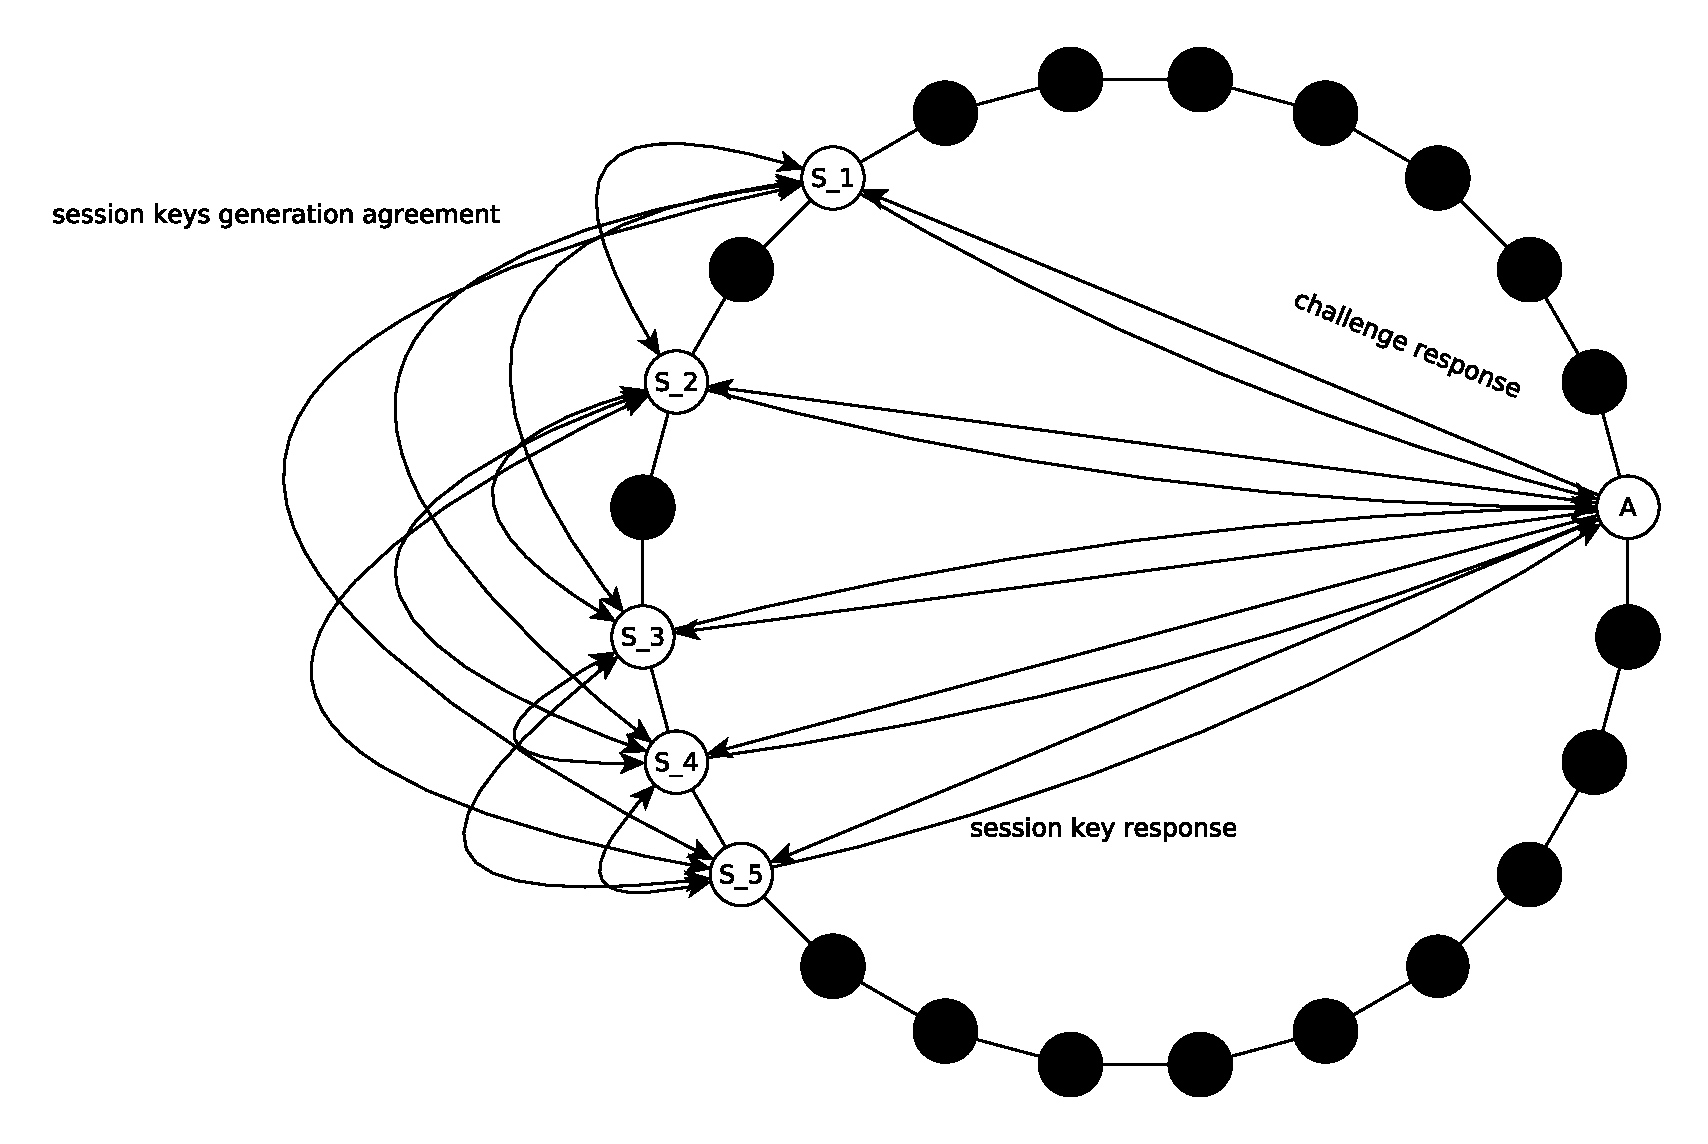
\includegraphics[height=0.7\textheight]{../../img/sign_in_3}\\
%\begin{table}
%\begin{tabular}{p{7cm}p{3cm}}
%&
%\vspace{1.5cm}
%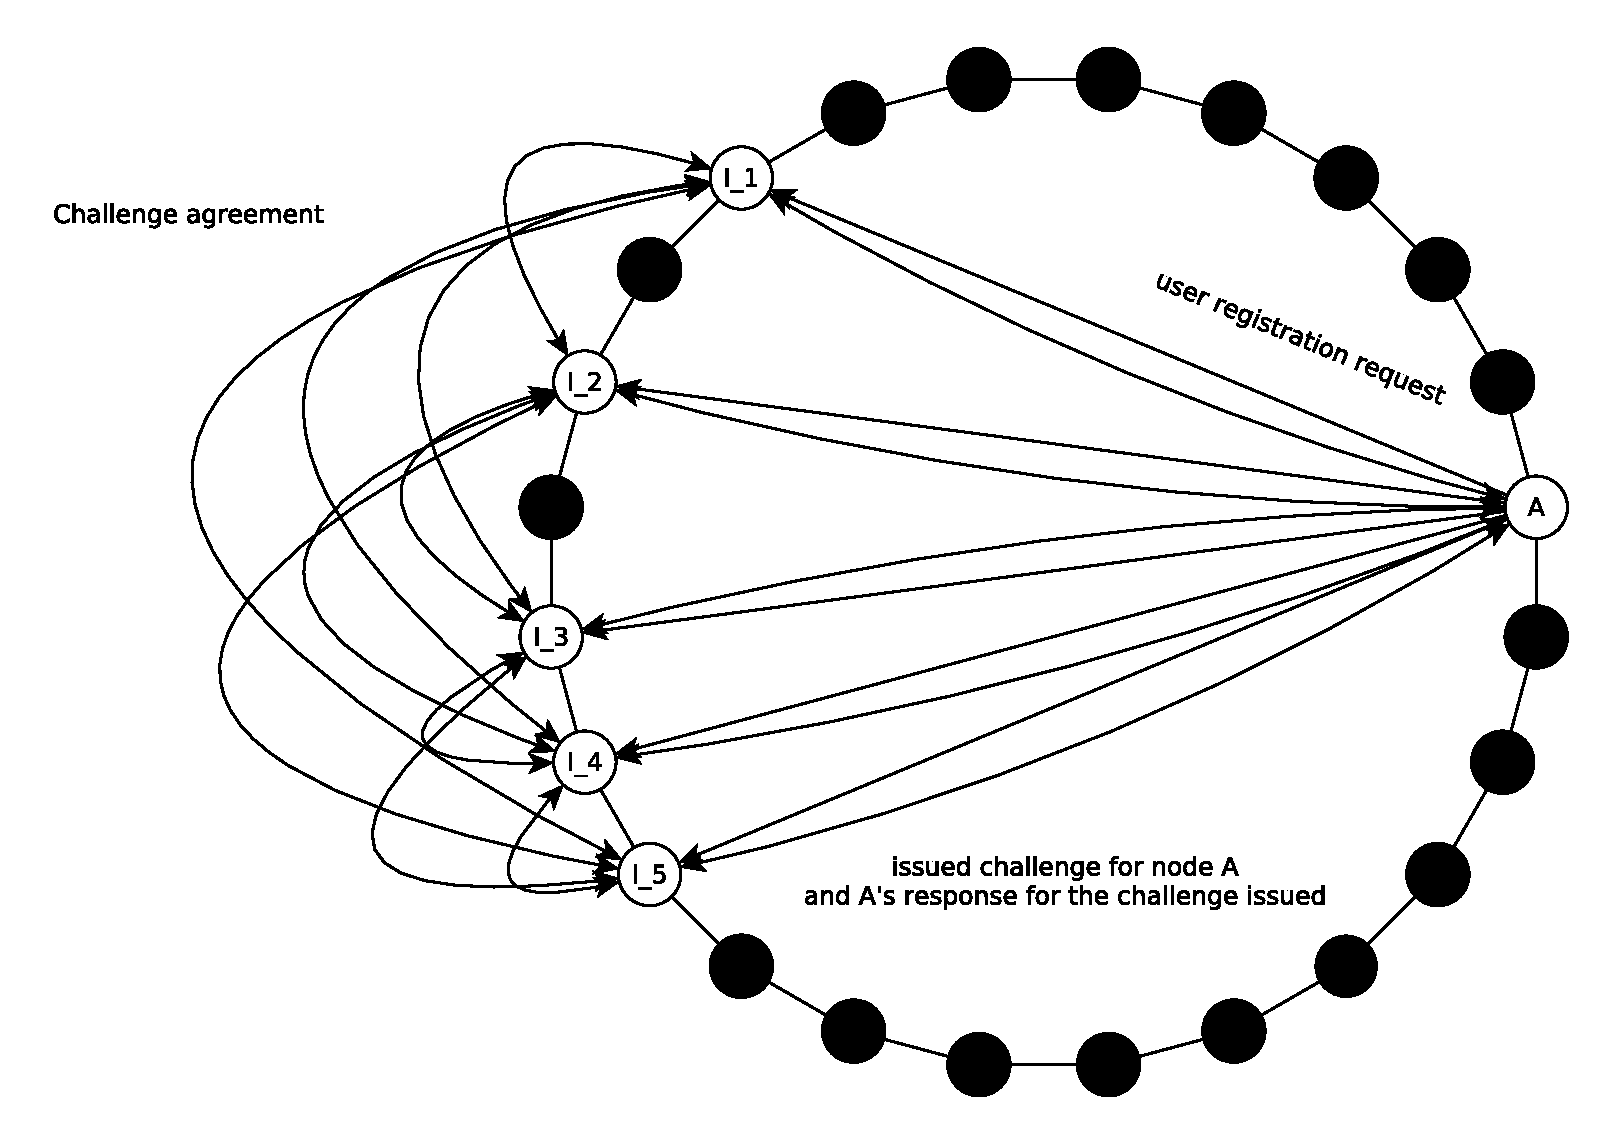
\includegraphics[width=4cm]{../../img/sign_up}\\
%\end{tabular}
%\end{table}
\end{frame}


\subsection{Logout, password change, user private key recovery}
\begin{frame}
\frametitle{System protocols}
\framesubtitle{More protocols}
\begin{table}
\begin{tabular}{p{7cm}p{3cm}}
\begin{itemize}
  \item Logout
  \item Password Change
  \item User private key recovery
\end{itemize}
&
\vspace{1.5cm}
%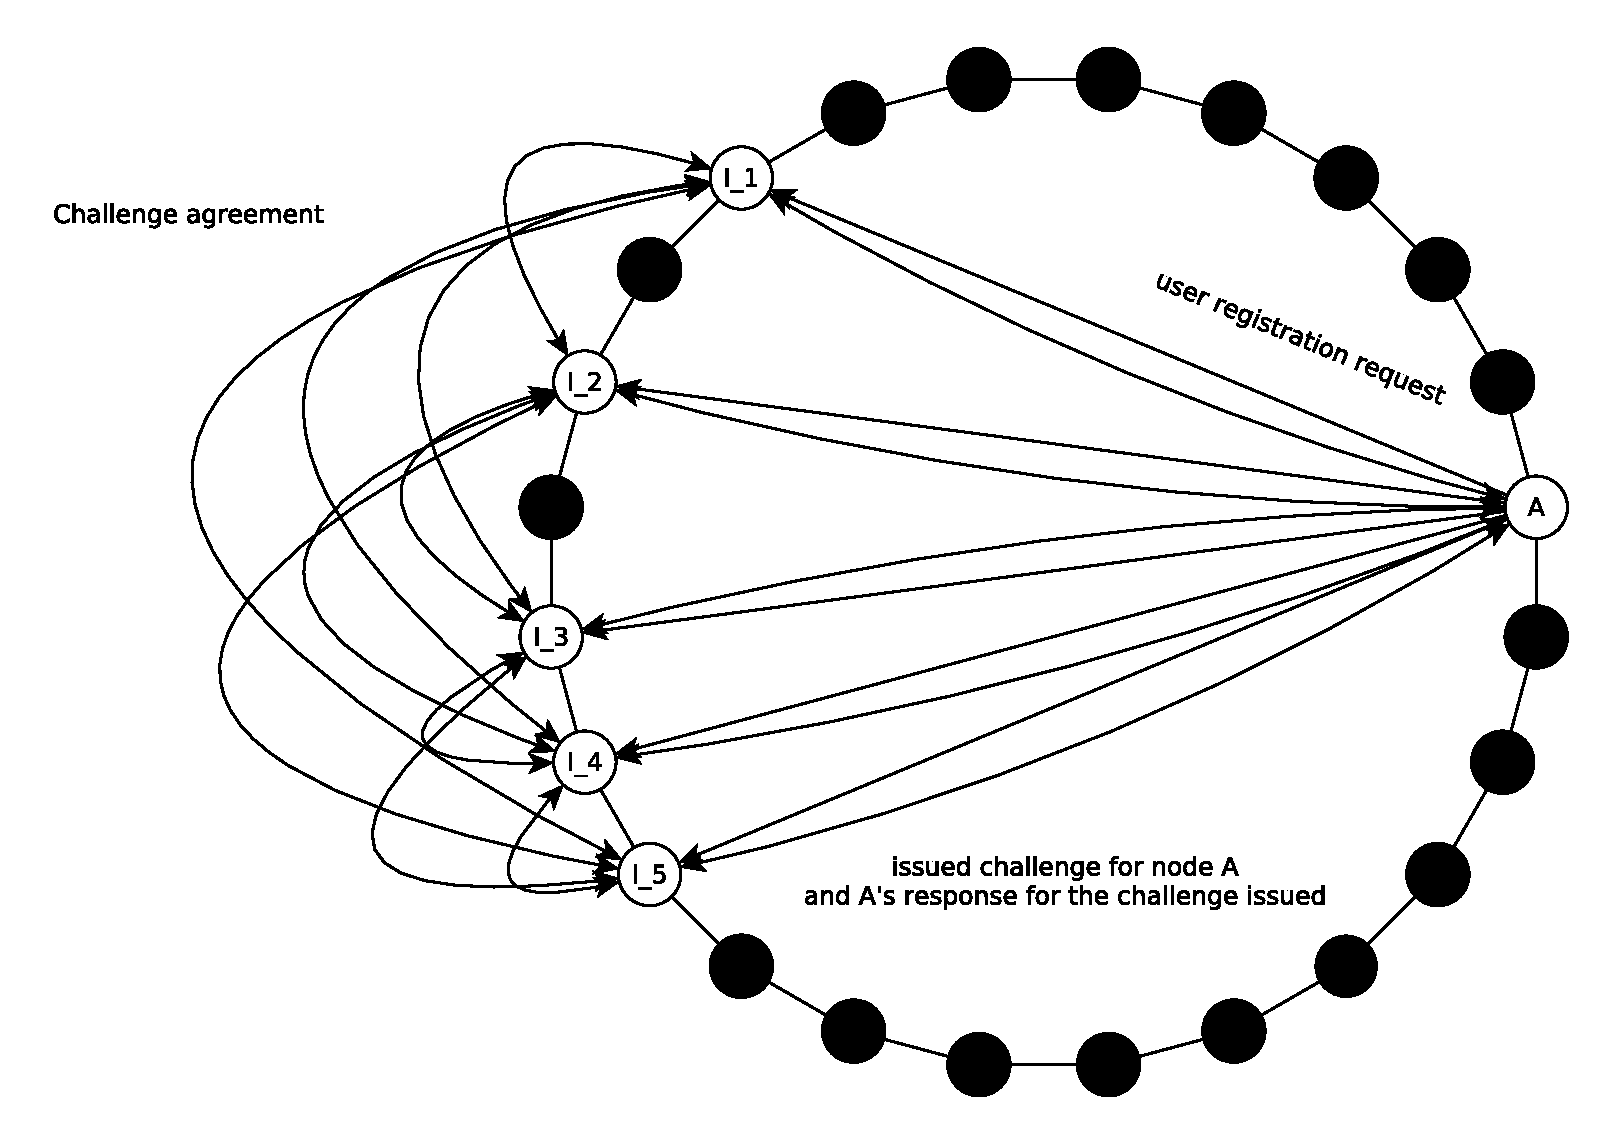
\includegraphics[width=4cm]{../../img/sign_up}\\
\end{tabular}
\end{table}
\end{frame}

\section{Evaluation}
\subsection{Parameters}
\begin{frame}
\frametitle{Evaluation}
\framesubtitle{Parameters}
  \begin{table}
    \centering
    \footnotesize
    \begin{tabular}{|ccc|}
      \hline
      \textbf{Parameter} & \textbf{Description} & \textbf{Value} \\
      \hline
      $\rho$ &  Probability of a node being malicious  & $0.3$  \\
      $\varepsilon$& CORPS classification error   & $0.05$ \\
      L &  Leafset/trustset size & $8$, $16$ or $32$  \\
      N &  Number of nodes in the DHT & $100000$  \\
      \hline
    \end{tabular}
    \caption{Parameters used for the evaluation of the protocols}
    \label{tab:variables_used}
  \end{table}
\end{frame}


\subsection{Probabilities of error}
\begin{frame}
\frametitle{Evaluation}
\framesubtitle{Probability of a system error/ protocol failure}
  \begin{table}
    \centering
    \footnotesize
    \begin{tabular}{|ccc|}
      \hline
      \textbf{Cases} & \textbf{System params} & \textbf{p value} \\
      \hline
      Worst case, no trusted nodes &  $L=8$  & $0.188$  \\
      Best case, no trusted nodes &  $L=32$  & $0.016$ \\
      Worst case, using trusted nodes &  $L=8$  & $6.64 \times 10^{-5}$ \\
      Worst case, using trusted nodes &  $L=32$  & $8.24 \times 10^{-14}$\\
      \hline
    \end{tabular}
    %\caption{Parameters used for the evaluation of the protocols}
    %\label{tab:variables_used}
  \end{table}
\end{frame}



\begin{frame}
\frametitle{Findings}
\framesubtitle{Theoretical results}
\begin{table}
\begin{tabular}{p{8cm}p{2cm}}
\begin{itemize}
  \item \textbf{Without trusted nodes:} With $p = 0.016$,\\
    \textbf{16000/1,000,000} failed transactions
  \item \textbf{Using a trusted set:} With $p =8.24 \times 10^{-14}$\\
    \textbf{0.00000000824/1,000,000} failed transactions
\end{itemize}
&
%\vspace{1.5cm}
%
\includegraphics[width=4cm]{img/example}\\
\end{tabular}
\end{table}
\end{frame}

%
%\begin{frame}
%\frametitle{Findings}
%\framesubtitle{Theoretical results}
%\begin{table}
%\begin{tabular}{p{7cm}p{3cm}}
%\begin{itemize}
%  \item A system with $1000000$ users, with the probability
%of a protocol failure being $p = 0.016$,  $16000$ of the users will have problems with
%the protocols of the system. In comparison, with a probability of $p =8.24 \times
%10^{-14}$, of $1000000$ transactions only $0.00000000824$ would fail.
%\end{itemize}
%&
%\vspace{1.5cm}
%
\includegraphics[width=4cm]{img/example}\\
%\end{tabular}
%\end{table}
%\end{frame}
%

\subsection{Conclusions}
\begin{frame}[allowframebreaks]
\frametitle{Conclusions}
\begin{itemize}
    \item while a 100\% secure implementation cannot be achieved, a viable solution exists.
    \item probability of error on the order of $10^{-14}$ can be achieved with a leafset size of $l = 32$.
    \item the system remains scalable.
    \framebreak
    \item the use of a reputation system and trusted nodes management mitigated the effectiveness of malicious node attacks in the network.
    \item a reputation system can also efficiently mitigate the effect of collusion attacks.
    \item computational challenges mitigate the problem of a node registering multiple users with the system.
      % reduce the probability from x to y? how this works?
%% comments
  % the system maintains a scalable cost when the size of nodes $n$ in the dht increases.
\end{itemize}
\end{frame}
